\documentclass[conference]{IEEEtran}
\IEEEoverridecommandlockouts
% The preceding line is only needed to identify funding in the first footnote. If that is unneeded, please comment it out.
\usepackage{cite}
\usepackage{amsmath,amssymb,amsfonts}
\usepackage{algorithmic}
\usepackage{graphicx}
\usepackage{textcomp}
\usepackage{xcolor}
\def\BibTeX{{\rm B\kern-.05em{\sc i\kern-.025em b}\kern-.08em
    T\kern-.1667em\lower.7ex\hbox{E}\kern-.125emX}}
\begin{document}

\title{Comparison of two selected ML models for predicting deaths due to COVID-19 outbreak}

\author{\IEEEauthorblockN{1\textsuperscript{st} Szymon Krasuski}
\IEEEauthorblockA{\textit{Warsaw University of Technology} \\
Warsaw
}
\and
\IEEEauthorblockN{2\textsuperscript{nd} Janusz Mikłuszka}
\IEEEauthorblockA{\textit{Warsaw University of Technology} \\
Czeladź
}
}


\maketitle

\begin{abstract}
COVID-19 outbreak gave forecasting models more popularity. People want to know when will it end and whether it can be predicted.
Autoregression models prove useful achieving this task. They can predict based on previous values of the time series.
Firstly we are checking wheter our data can be used to train AR model. We achieve this using autocorrelation plots and lag plots.
We developed dash application to show forecasting results. In the app it is possible to set horizon of prediction, source data and prediction model.


\end{abstract}

\begin{IEEEkeywords}
COVID-19, Machine learning, Autoregression.
\end{IEEEkeywords}

\section{Introduction}
Current coronavirus pandemic started in chinese Wuhan, in December 2019. On 11 March WHO made the assessment that COVID-19 can be
 characterized as pandemic which became global problem. On 4 March first case in Poland appeared. From this time number of confirmed cases was steadily increasing.
 Month later there was 5000 confirmed cases.

\section{Problem Description}
Using databases of confirmed cases, death cases and recovered cases of COVID-19 we can create model which can give us predictions of future cases.
 Based on these prediction decisions can be made regarding public restrictions and other regulations.

 \begin{figure}[h!]
    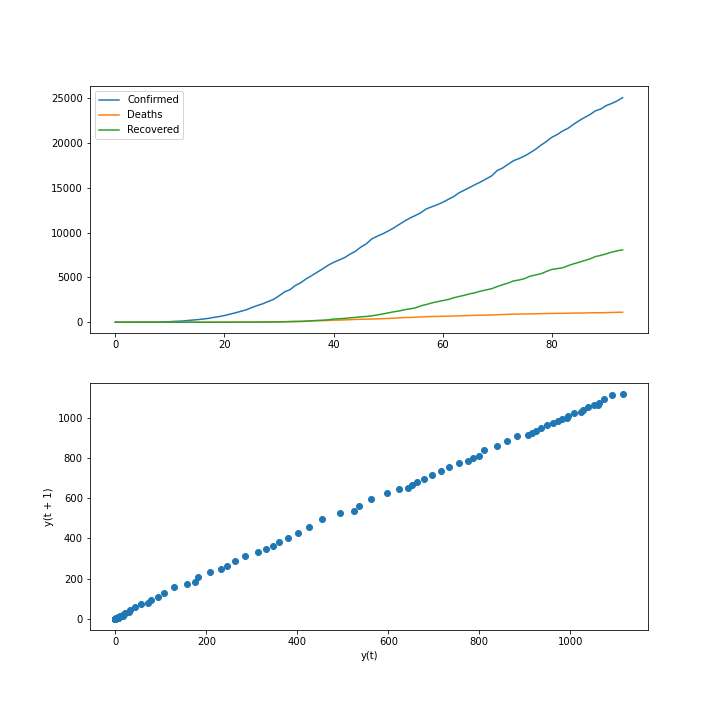
\includegraphics[width=\linewidth]{images/Correlation_lag_Deaths.png}
    \caption{a) Time series of confirmed, death and recovered cases. b) Lag plot of death cases}
    \label{fig:lag_plot}
\end{figure}

The time series plot indicates relationship among the series. Linear shape of lag plot suggest positive autocorrelation between next values of death cases.
 This suggest that using autoregression (AR) model is good choice.
Randomness of the time series can be checked by autocorrelation plot of the time series. 

\begin{figure}[h!]
    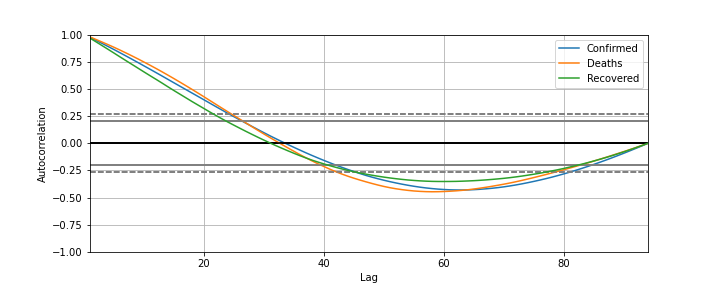
\includegraphics[width=\linewidth]{images/AutoCorrelation.png}
    \caption{Autocorrelation of the time series}
    \label{fig:AutoCorrelation}
\end{figure}

For non-random time series autocorrelations are significantly non-zero. Above figure shows that lag values about 10 are worth considering. 
 Such high autocorrelation values further proves viability of AR model.

There might be also relation of death cases with confirmed and recovered cases. Pairplot confirms our suspicion showing high correlation with both of them

\begin{figure}[h!]
    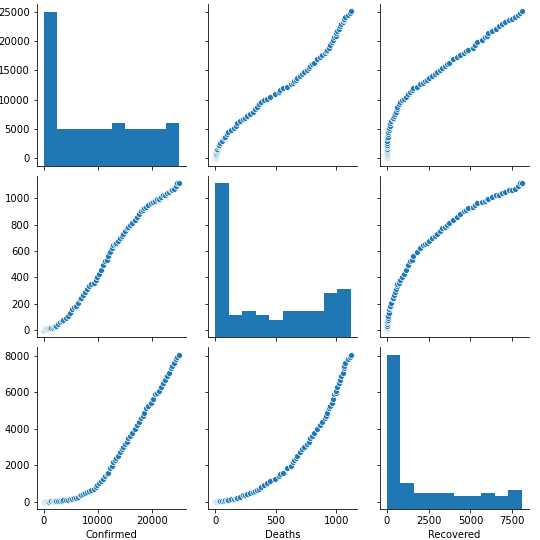
\includegraphics[width=\linewidth]{images/Correlation.png}
    \caption{Autocorrelation of the time series}
    \label{fig:AutoCorrelation}
\end{figure}

To take that variables into account during our predictions VAR model can be used.
 To use VAR model data two assumptions are needed:
 \begin{itemize}
\item all variables must be Stationary,
\item there exist a linear relation between their current and past values
\end{itemize}

\begin{figure}[h!]
    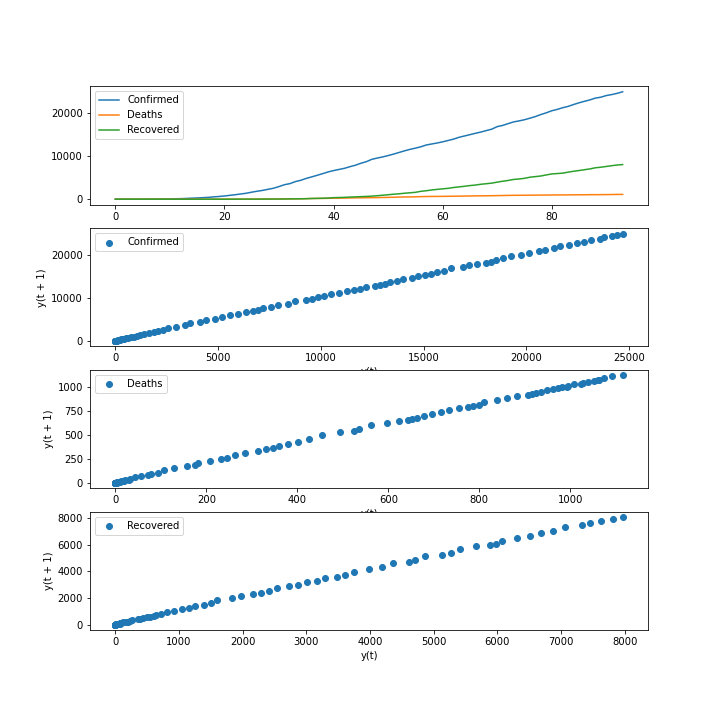
\includegraphics[width=\linewidth]{images/Correlation_lag.png}
    \caption{Autocorrelation of the time series}
    \label{fig:AutoCorrelation}
\end{figure}

Above figure confirms relation between values. Augmented Dickey-Fuller Test is used to check stationarity. If the result of the test indicates that data is non-stationary,
then data connot be used. Fortunately a difference transform is good way of remowing a systematic structure from time series. It can be done by using
 pandas.DataFrame.diff().dropna() method. It can be done second time when ADF test is still negative.


\section{Domain Implementation}
% tego nie jestem pewien co powinno być, może coś w czym robimy
We are using Python enviroment to create application which based on provided data and prediction horizon, makes predictions of number of deaths per day.

Project structure is organised into consistent class which implements methods for gathering data, training machine learning model and data visualization.
\newline
\newline
Data gathering is separate module that allows to download data in the runtime from provided web server or load data from local file.
Data format has to be consistent with format provided by user dtandev in repository "coronavirus" published on GitHub platform.
Data is presented as summarized numbers per columns starting from 3rd March 2020.
Because of that data gathering module on reading raw data has additonal steps which
detects which one of two supported formats are used in data.
Currently project supports data presented in csv files with columns named as data presented in GitHub repositories anuszka/COVID-19-MZ\_GOV\_PL or dtandev/coronavirus.
These two repositories were originally choosen as source of data for machien learning model.
Additonaly, data is parsed to return only columns containing dates and day-to-day deaths which are calculated from summarized deaths since start of pandemic.
Complete data is returned in Pandas DataFrame.
\newline
\newline
Main class contain methods which implement steps easy to split for external resources e.g. GUI applications:
\begin{itemize}
\item \textit{load\_data} - implements data gathering model to load data from web or local file. It is possible to provide data also as complete DataFrame during object initialization.
\item \textit{set\_predict\_horizon} - sets dates in which next data points should be predicted. Dates should be datatime object from datatime library.
\item \textit{train\_AR} - method which trains Autoregression model based on previously loaded data.
\item \textit{train\_VAR} - method which trains Vector Autoregression model based on previously loaded data.
\item \textit{predict} - Because it is possible to alternatively train model with two separate methods then this method uses one of models (the one that was run as last) and predicts next data points up to predict horizon.
\item \textit{plt} - this method prints out matplotlib plot with actual data and predicted data points.
\item \textit{get\_dcc\_Graph} - this method returns Dash Core Components Graph with actual data and predicted data which may be used with GUI applications created in Dash
\end{itemize}
Presented project utilizes Dash library in order to implement user-friendly application.
\begin{figure}[h!]
    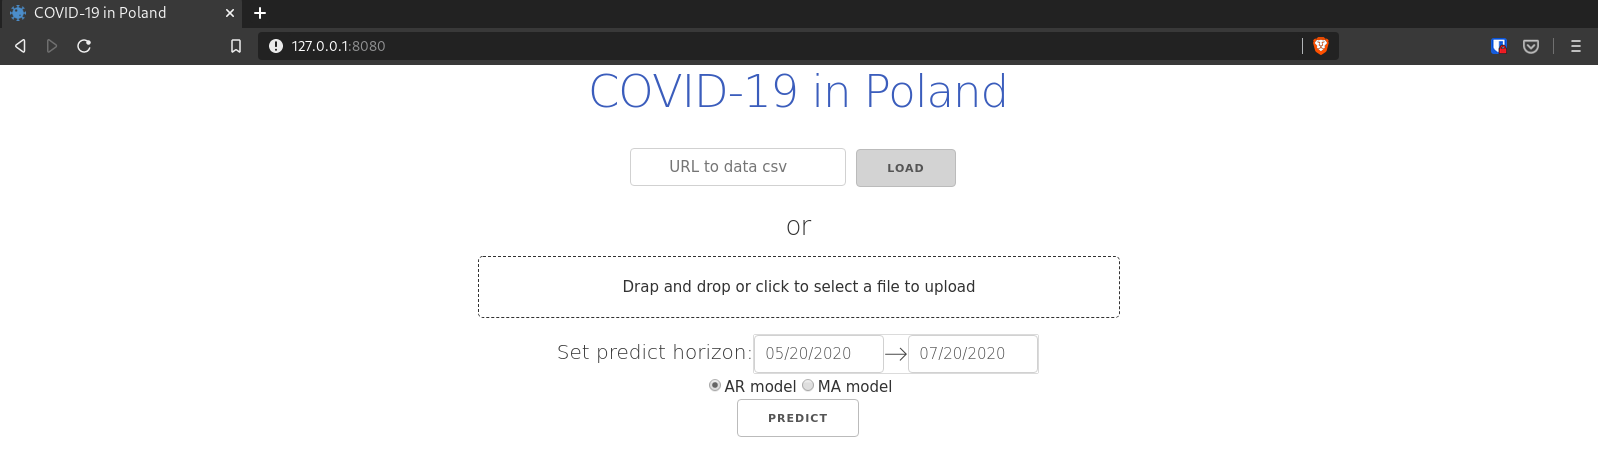
\includegraphics[width=\linewidth]{images/gui1.png}
    \caption{User welcome screen}
    \label{fig:gui1}
\end{figure}
\newline
User at the first site layout have simple control which allow to load data from pasted URL (by default URL to data from dtandev/coronavirus repository is available to choose from text field) or local file.
Afterwards, user has possiblity to set data which will be used as predict horizon adn finally choose one of two training models.
\newline
When user clicks 'Predict' button then below is generated interactive Dash Core Component Graph.
\begin{figure}[h!]
    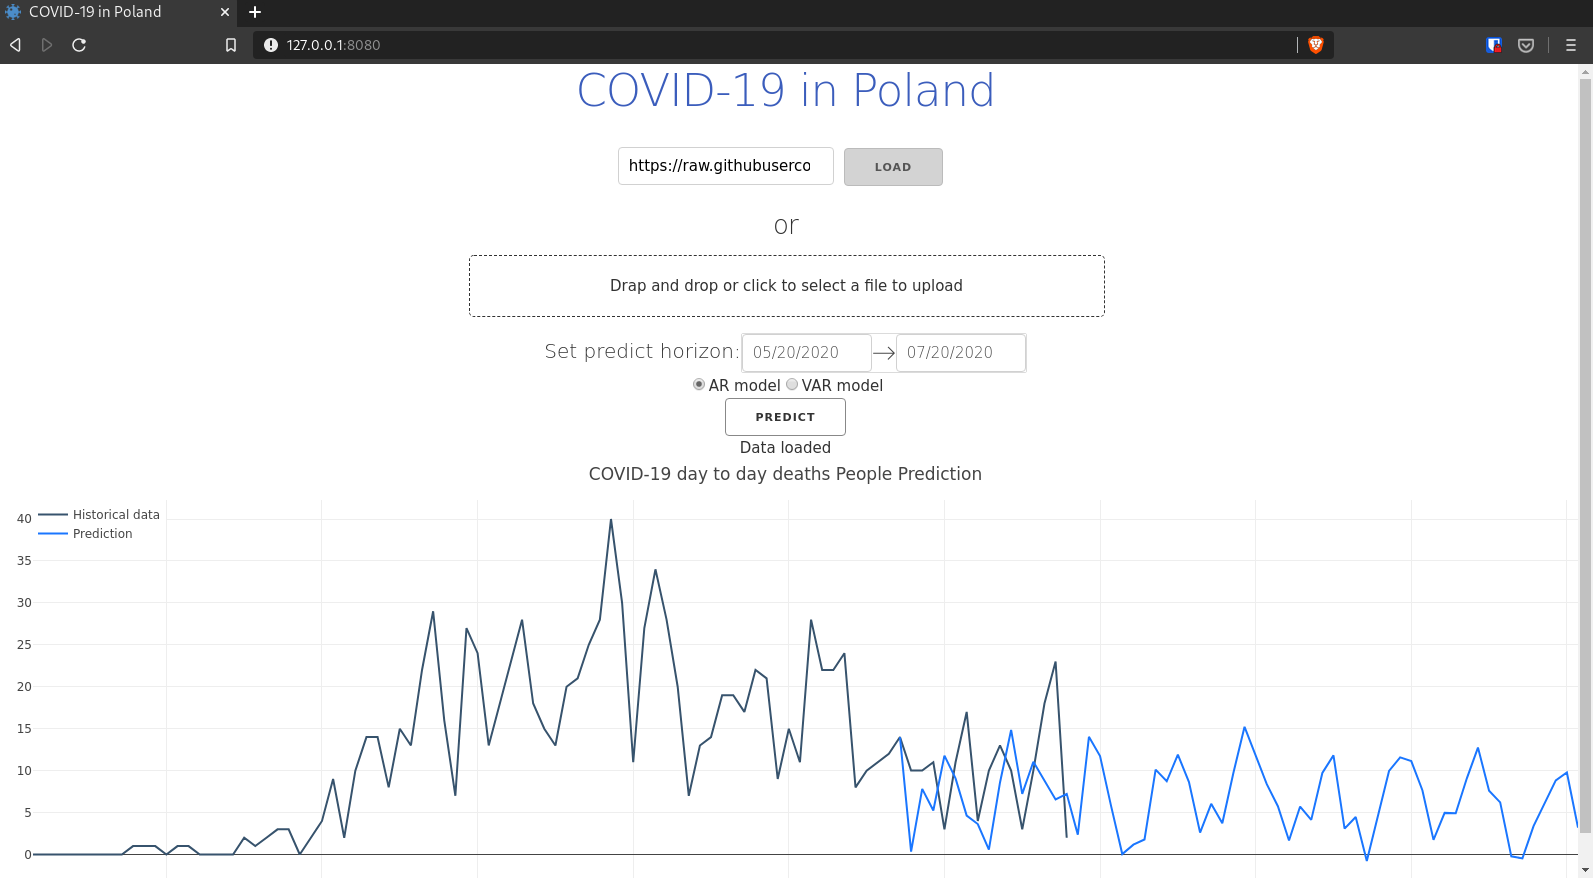
\includegraphics[width=\linewidth]{images/gui2.png}
    \caption{Application after setting parameters and prediction process}
    \label{fig:gui2}
\end{figure}
\newline
User has always possiblity to modify parameters and repeat prediction from any point of process.
\newline
\newline
Whole project is covered with unit tests which are used as regression tests for project to make sure that with every code edition all other components still work properly.
\newline
Tests are run automatically in every Pull Request created on GitHub platform of project (currently private repository) with CircleCI platform.
\newline
Test job was created with tox tool which contains two test jobs.
\newline
One runs unit tests and second one run flake8 command which tests code compability with PEP8 standard.

\section{Machine Learning Models}
\subsection{AutoReg}
We are using AutoReg function from statsmodel library. 
 It is primarily used  to describe time-varying processes in nature. This type of model specifies the output
  variable based on its previous values and stochastic term. Along with moving-average (MA) model it is component of more general autoregressive-moving-average
  model (ARMA). Dynamic of the autoregressive model of order p AR(p) is given by:
\begin{equation}
    X_t = c + \sum_{i=1}^{p} (\phi_iX_{t-i}) + \epsilon_t
\end{equation}
where
p - order of the model\newline
$ \phi $ - parameters of the model\newline
c - constant\newline
$\epsilon_t$ - white noise\newline

\subsection{ARMA}
It is simirial to AR model. MA part involves modeling the error term as linear combination of error terms  occurring contemporaneously and at various times in the past.


Moving average model of order q MA(q) is written:
\begin{equation}
    X_t = \mu + \epsilon_t + \sum_{i=1}^{q} (\theta_i\epsilon_{t-i})
\end{equation}

ARMA(p,q) notation refers to AR(p) and MA(q) models:
\begin{equation}
    X_t = c + \epsilon_t +\sum_{i=1}^{p} (\phi_iX_{t-i}) + \sum_{i=1}^{q} (\theta_i\epsilon_{t-i})
\end{equation}

\subsection{VAR}
Vector autoregression is a stochastic process model used to capture the linear interdependencies among multiple time series. It generalizes univariate AR model by allowing more 
than one evolving variable. All variables have an equation explaining its evolution based on its own lagged values.

\section{Results}
Predictions done by AR model are presented below

\begin{figure}[h!]
    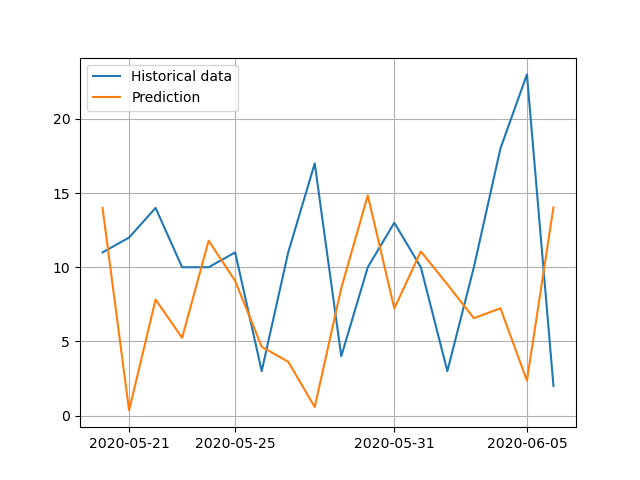
\includegraphics[width=\linewidth]{images/AR_pred.png}
    \caption{AR model predictions}
    \label{fig:AR_pred}
\end{figure}
Mean Squared Error is 75.069 and Mean Absolute Error is 6.875. 

For VAR model predictions are less accurate as presented below
\begin{figure}[h!]
    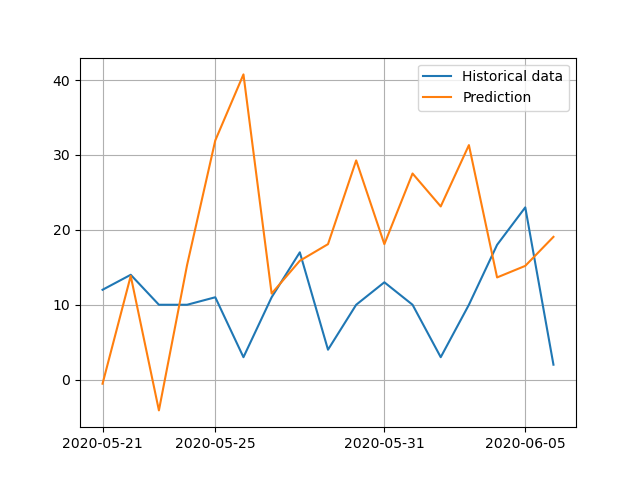
\includegraphics[width=\linewidth]{images/VAR_pred.png}
    \caption{VAR model predictions}
    \label{fig:VAR_pred}
\end{figure}
Mean Squared Error is 46758.033 and Mean Absolute Error is 63.003. Not only this model needs more resources but it produces worse results.


\section{Summary}
It's fairly easy to create prediction model for COVID-19 data. But model needs more finetunnig to be accurate. Also it can not forecast big outbursts. These deviations can lead to 
bad predictions. Both models are susceptible to these as death and recovered cases are mainly influenced by number of confirmed cases.


\begin{thebibliography}{00}
\bibitem{b1} Prediction of multivariate time series by autoregressive model fitting, Richard Lewis, Gregory CReinsel, 1985, https://www.sciencedirect.com/science/article/pii/0047259X85900272
\bibitem{b2} Autoregressive Model Fitting for Control, Hirotugu Akaike, 1970, https://link.springer.com/chapter/10.1007/978-1-4612-1694-0\_12
\bibitem{b3} RainFARM: Rainfall Downscaling by a Filtered Autoregressive Model, Nicola Rebora, Luca Ferraris, 2005, https://journals.ametsoc.org/doi/full/10.1175/JHM517.1
\bibitem{b4} https://github.com/dtandev/coronavirus
\bibitem{b5} https://github.com/anuszka/COVID-19-MZ\_GOV\_PL
\bibitem{b6} Time-series Analysis with VAR and VECM: Statistical approach, Sarit Maitra, 2019, https://towardsdatascience.com/vector-autoregressions-vector-error-correction-multivariate-model-a69daf6ab618
\bibitem{b7} Time Series Forecasting using Granger’s Causality and Vector Auto-regressive Model, Sarit Maitra, 2019, https://towardsdatascience.com/granger-causality-and-vector-auto-regressive-model-for-time-series-forecasting-3226a64889a6
\end{thebibliography}
\vspace{12pt}

\end{document}
